
\documentclass{beamer}
\usetheme{ucl}

%%% Increase the height of the banner: the argument is a scale factor >=1.0
%\setbeamertemplate{banner}[ucl][0.1]

%%% Change the colour of the main banner
%%% The background should be one of the UCL colours (except pink or white):
%%%   black,darkpurple,darkred,darkblue,darkgreen,darkbrown,richred,midred,
%%%   navyblue,midgreen,darkgrey,orange,brightblue,brightgreen,lightgrey,
%%%   lightpurple,yellow,lightblue,lightgreen,stone
\setbeamercolor{banner}{bg=darkpurple}
%\setbeamercolor{banner}{bg=yellow,fg=black}

%%% Add a stripe behind the banner
%\setbeamercolor{banner stripe}{bg=darkpurple,fg=black}

%%% The main structural elements
\setbeamercolor{structure}{fg=black}

%%% Author/Title/Date and slide number in the footline
\setbeamertemplate{footline}[author title date]

%%% Puts the section/subsection in the headline
% \setbeamertemplate{headline}[section]

%%% Puts a navigation bar on top of the banner
%%% For this to work correctly, the each \section command needs to be
%%% followed by a \subsection. Requires one extra compile.
% \setbeamertemplate{headline}[miniframes]
%%% Accepts an optional argument determining the width
% \setbeamertemplate{headline}[miniframes][0.3\paperwidth]


%%% Puts the frame title in the banner
%%% Won't work correctly with the above headline templates
%\useoutertheme{ucltitlebanner}
%%% Similar to above, but smaller (and puts subtitle on same line as title)
\useoutertheme[small]{ucltitlebanner}

%%% Gives block elements (theorems, examples) a border
% \useinnertheme{blockborder}
%%% Sets the body of block elements to be clear
% \setbeamercolor{block body}{bg=white,fg=black}

%%% Include CSML logo on title slide
%\titlegraphic{\includegraphics[width=0.16\paperwidth]{csml_logo}}

%%% Include CSML logo in bottom right corner of all slides
%\logo{\includegraphics[width=0.12\paperwidth]{csml_logo}}

%%% Set a background colour
% \setbeamercolor{background canvas}{bg=lightgrey}

%%% Set a background image
%%% Some sample images are available from the UCL image store:
%%%   https://www.imagestore.ucl.ac.uk/home/start
% \setbeamertemplate{background canvas}{%
%   \includegraphics[width=\paperwidth]{imagename}}



%%%%%% Some other settings that can make things look nicer
%%% Set a smaller indent for description environment
\setbeamersize{description width=2em}
%%% Remove nav symbols (and shift any logo down to corner)
\setbeamertemplate{navigation symbols}{\vspace{-2ex}}








\DeclareMathOperator{\Cov}{Cov}
\DeclareMathOperator{\Var}{Var}
\DeclareMathOperator{\E}{\mathbb{E}}
\DeclareMathOperator{\Proba}{\mathbb{P}}

\newcommand{\Covb}[2]{\ensuremath{\Cov\!\left[#1,#2\right]}}
\newcommand{\Eb}[1]{\ensuremath{\E\!\left[#1\right]}}
\newcommand{\Pb}[1]{\ensuremath{\Proba\!\left[#1\right]}}
\newcommand{\Varb}[1]{\ensuremath{\Var\!\left[#1\right]}}

% norm
\newcommand{\norm}[1]{\| #1 \|}

\newcommand{\indep}{\rotatebox[origin=c]{90}{$\models$}}





\usepackage{mathptmx,amsmath,amssymb,graphicx,bibentry,bbm,ragged2e}
\usepackage[english]{babel}

\makeatletter

\newcommand{\noun}[1]{\textsc{#1}}
\newcommand{\jitem}[1]{\item \begin{justify} #1 \end{justify} \vfill{}}
\newcommand{\sframe}[2]{\frame{\frametitle{#1} #2}}

\newenvironment{centercolumns}{\begin{columns}[c]}{\end{columns}}
%\newenvironment{jitem}{\begin{justify}\begin{itemize}}{\end{itemize}\end{justify}}



%\usetheme{Warsaw}
%\setbeamertemplate{footline}[text line]{}
%\setbeamertemplate{headline}{}
%\setbeamercolor{structure}{fg=purple!50!blue, bg=purple!50!blue}

%\setbeamersize{text margin left=15pt,text margin right=15pt}

%\setbeamercovered{transparent}


\@ifundefined{showcaptionsetup}{}{%
 \PassOptionsToPackage{caption=false}{subfig}}
\usepackage{subfig}

\usepackage[utf8]{inputenc}
\usepackage[T1]{fontenc}

\usepackage{multirow}


\makeatother

\def \draft {1}

\usepackage{xparse}
\usepackage{ifthen}
\DeclareDocumentCommand{\comment}{m o o o o}
{\ifthenelse{\draft=1}{
    \textcolor{red}{\textbf{C : }#1}
    \IfValueT{#2}{\textcolor{blue}{\textbf{A1 : }#2}}
    \IfValueT{#3}{\textcolor{ForestGreen}{\textbf{A2 : }#3}}
    \IfValueT{#4}{\textcolor{red!50!blue}{\textbf{A3 : }#4}}
    \IfValueT{#5}{\textcolor{Aquamarine}{\textbf{A4 : }#5}}
 }{}
}
\newcommand{\todo}[1]{
\ifthenelse{\draft=1}{\textcolor{red!50!blue}{\textbf{TODO : \textit{#1}}}}{}
}




\begin{document}

\title[Industrial symbiosis ABMs]{Agent-based models of industrial symbiosis networks}
\author[Raimbault, Serna Vazquez et al.]{J. Raimbault$^{1\ast}$, J.M. Serna Vazquez$^{2}$, J. Broere$^{3}$, M. Somveille$^{4}$, E. Strombom$^{5}$, C. Moore$^{6}$, B. Zhu$^{7}$, L. Sugar$^{8}$\\\medskip
$^{\ast}$\texttt{j.raimbault@ucl.ac.uk}
}

\institute[]{(1) CASA, UCL; (2) Universit{\'e} de Paris, CRPMS; (3) Utrecht University, Centre for Complex Systems Studies; (4) University of Oxford, Edward Grey Institute; (5) University of Minnesota, CBS Ecology; (6) University of Oxford, Environmental Change Institute; (7) Delft University of Technology, Department of Engineering Systems and Services; (8) University of Toronto, Department of Civil Engineering
}


\date[November 30th 2021]{Future Days 2021 - Session Circular Economy\\
November 30th 2021
}

\frame{\maketitle}



\section{Introduction}




\sframe{Questions}{

\justify

\textit{General: } How to use modern computer modeling tools to help foster circular economy by helping turn waste and by-products into resources, all the while generating economical incentives in the process?

\bigskip

\textit{Specific: } How can symbiotic exchanges between industries be optimized in terms of sustainability, given a set of actors located in a geographical area?


\bigskip

$\rightarrow$ We propose an agent-based model to evaluate optimal symbiotic exchanges of waste that may become a resource for compatible industries, all the while factoring their geographical position (which has an impact on the cost of transport for these exchanges).


}


\sframe{Our Model studies}{

\footnotesize

\begin{enumerate}
	\item The effect of geographical properties on symbiotic relationship by \textbf{minimizing both cost and waste products} (multi-objective optimization). The \textbf{system size} can be: \textbf{regional}, \textbf{national}, or even \textbf{global}.
	\item The dynamics of how symbiotic exchanges between enterprises are established with \textbf{linkages that grow organically}, thus \textbf{based on mutual benefit (``Win win!'') and geographical proximity, and not solely on central control.}
	\item Industries as complex systems: drawing on the transfer of concepts and models between ecology and industrial ecology, generative social science, pattern oriented modeling and geosimulation.
\end{enumerate}

\medskip

\centering

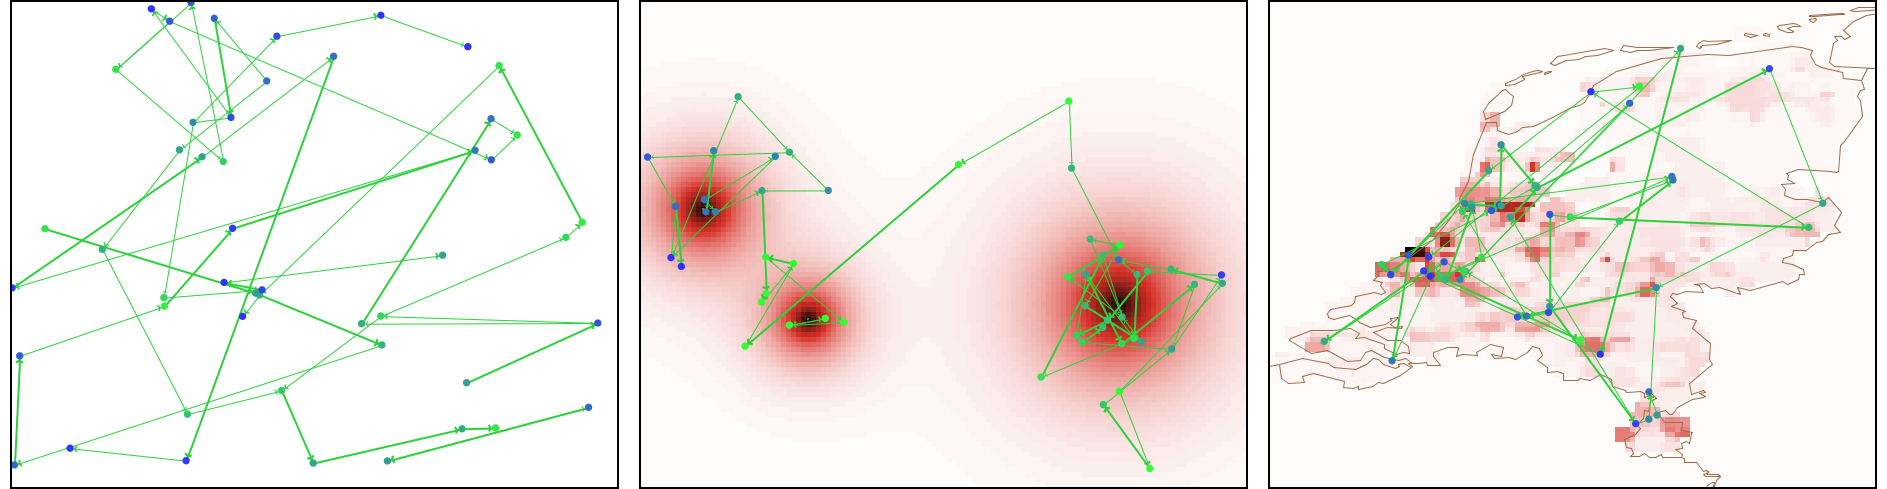
\includegraphics[width=\linewidth]{figures/Fig2.png}

}


\sframe{Benefits}{

\justify

$\rightarrow$ \textbf{Insights for identifying matching} complementary actors to \textbf{minimizing cost and waste products.}

\bigskip

$\rightarrow$ Understand how symbiotic linkages can be optimized given the geographical properties of an area.

\bigskip

$\rightarrow$ A macro perspective with potential uses for policy planning and sustainable urban planning, relying either on top-down approaches (planning) or on bottom-up processes (incentives to change the behavior at the company level) \cite{velenturf2016promoting}, as both aspects can be investigated with this model.

}


\sframe{Findings}{

%\footnotesize
\justify

$\rightarrow$ Introduction of the first agent-based spatial model for growing a symbiotic system at this scale.

\medskip

$\rightarrow$ Applying state-of-the-art model exploration and calibration techniques with high performance computing to extract knowledge on model behavior.

\medskip

$\rightarrow$ Identify stylized findings from model simulations that may have important implications for policy planning.

\medskip

$\rightarrow$ We show that the model can be applied and calibrated on a real world setting, thus having the ability to compare the findings to empirical and/or alternative scenarios.

\bigskip

\textbf{Future outcomes:}

$\rightarrow$ This work introduces a framework that can be used for studying both practical and theoretical questions, with future extensions being more data driven.

}


\sframe{Model details}{


\begin{columns}

\begin{column}{0.55\linewidth}

\tiny
\justify

 - Industrial plants are agents located in space with inputs and outputs that they can exchange. The industrial compatibility between outputs (waste) and inputs (resources) is determined by the overlap of probability distributions over a one-dimensional axis.

\medskip

 - The model is \textbf{spatially explicit: the closer two plants are, the higher the probability to interact.}

\medskip

 - Then, among potential partners (closer plants which are compatible - i.e. distribution overlap is over a threshold), \textbf{the exchange contract will be done with the neighbor with maximal utility}, where \textbf{the utility aggregates transportation costs and quantity of resources (overlap).}

\medskip

- This gives an exchange network that grows iteratively until it stabilizes.

\medskip

 - A focus on geographical proximity and industrial cluster is obtained with an additional process: one spatial correlation parameter is used to increase the compatibility of close plants, at model setup (by correlating their distribution average). A very high correlation corresponds to the implementation of local industrial parks.
\end{column}
 \begin{column}{0.45\linewidth}
 \centering
 
 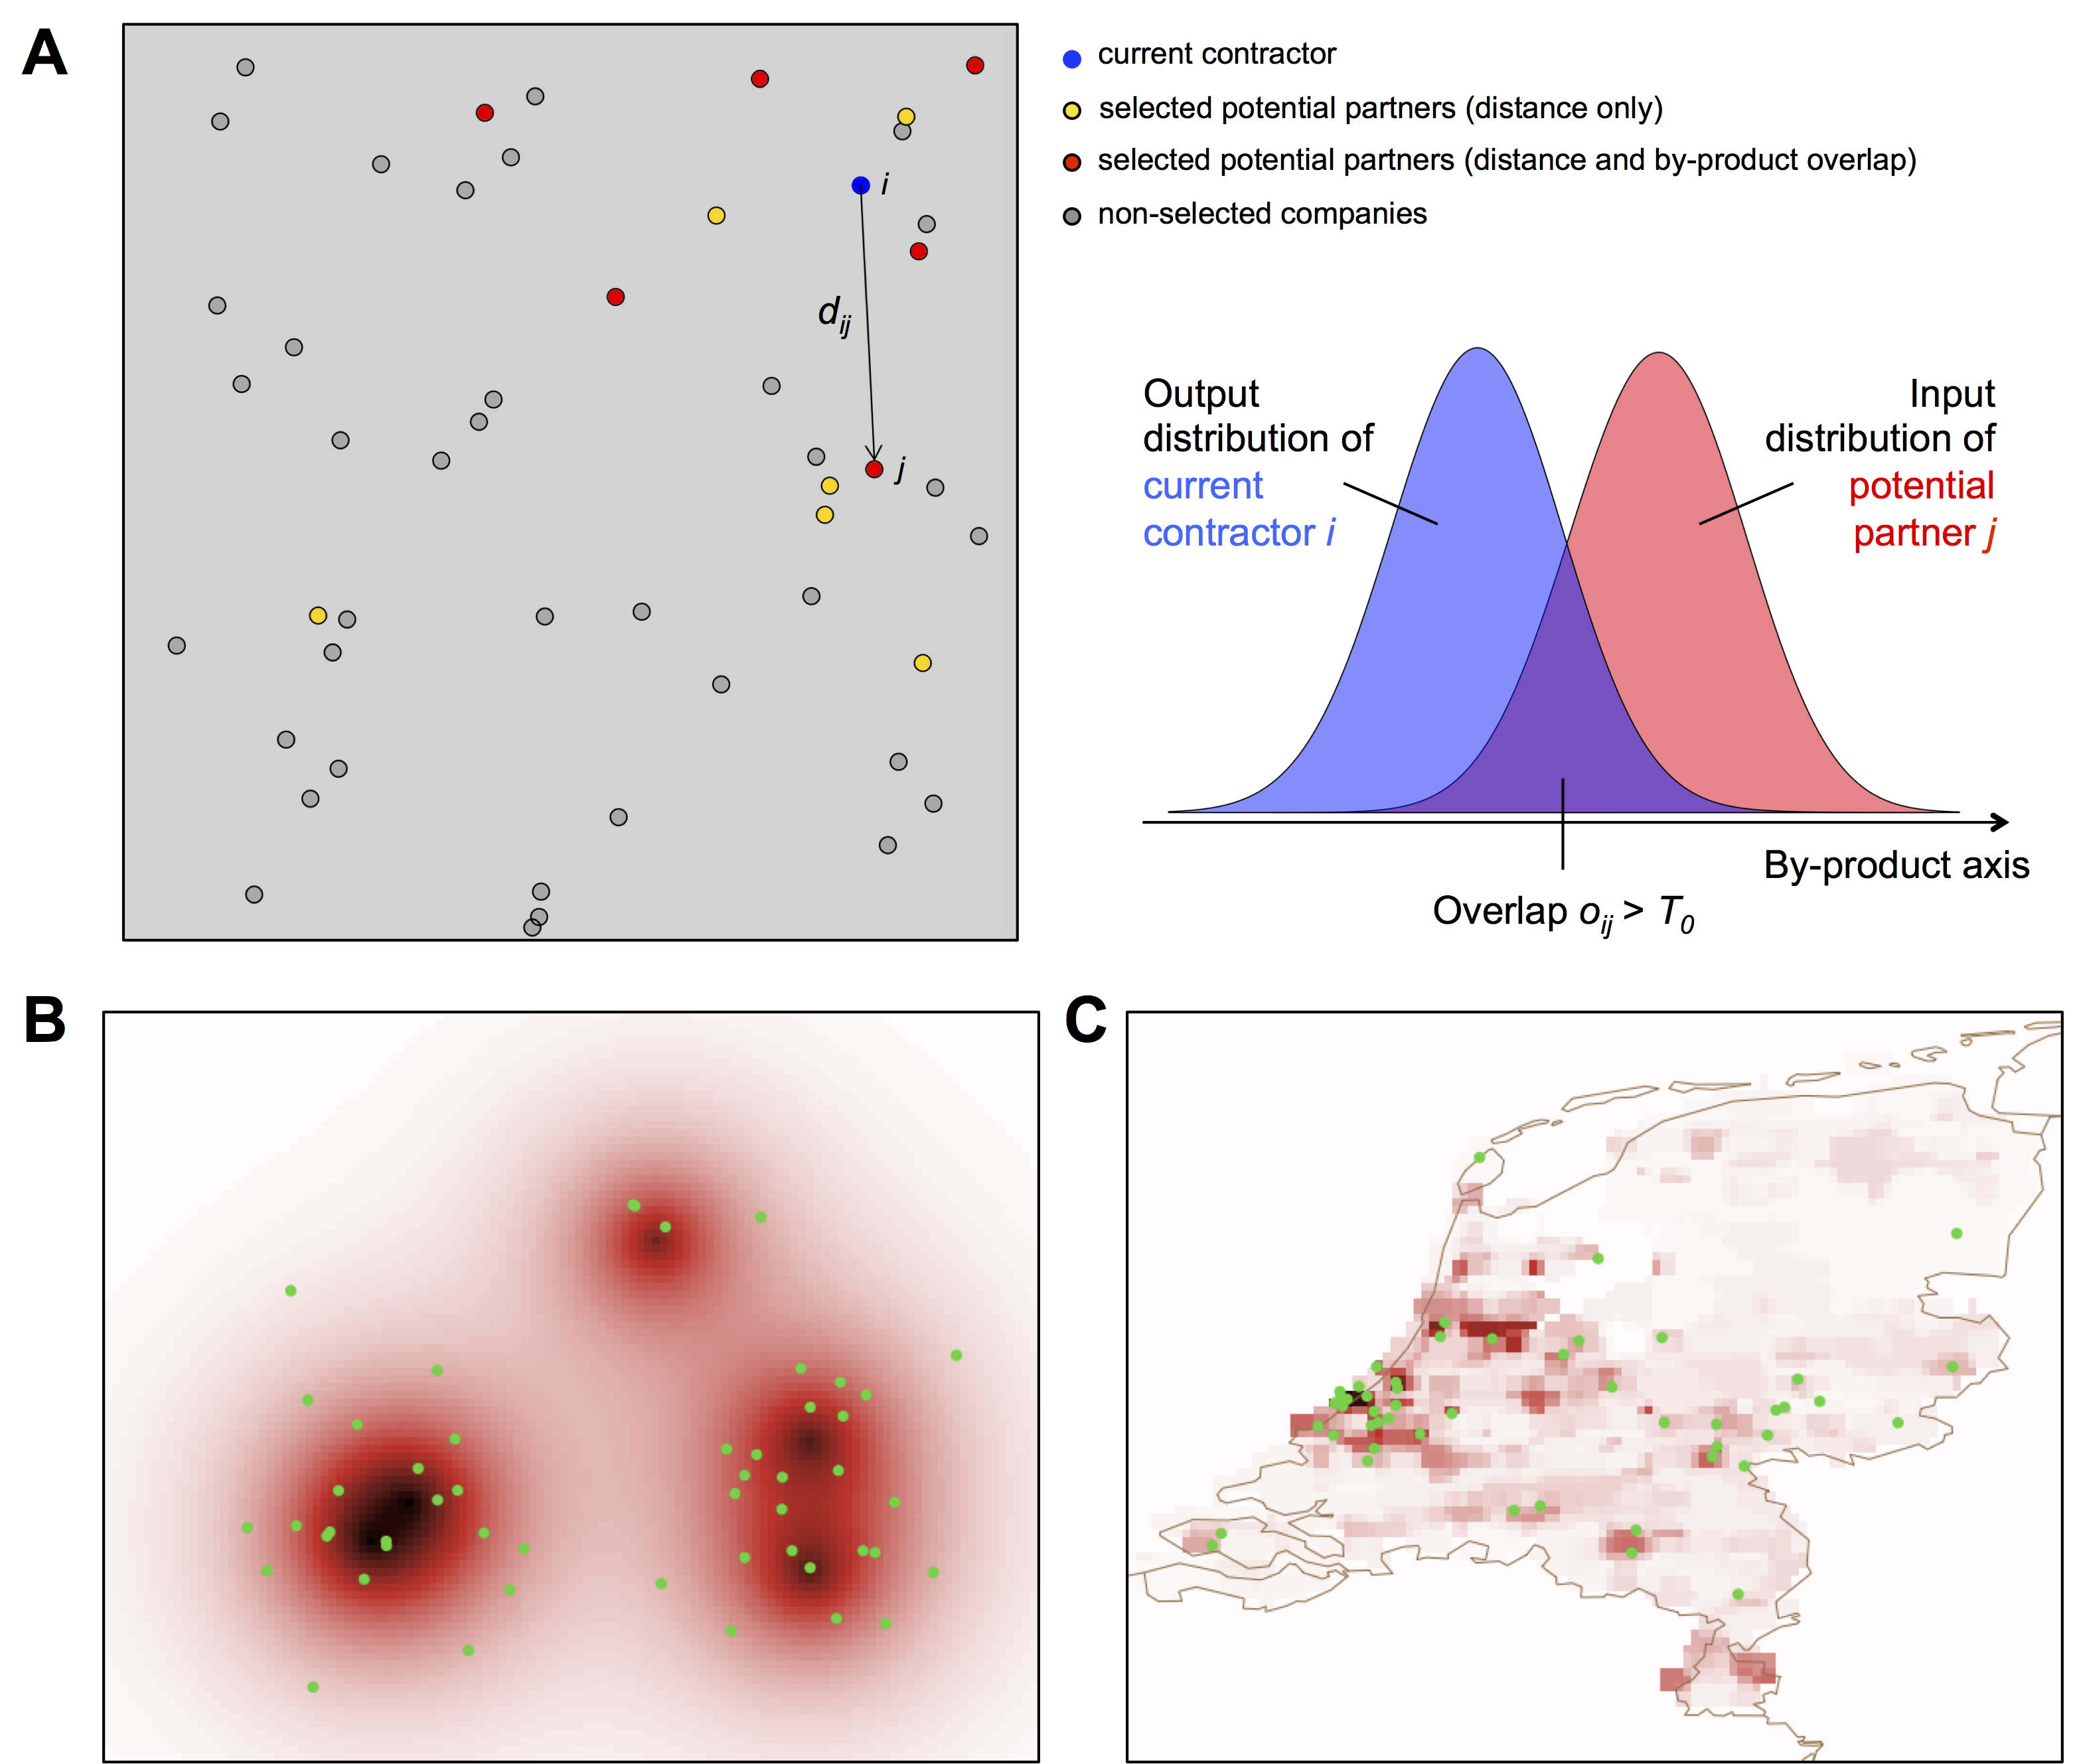
\includegraphics[width=\linewidth]{figures/Fig1.png}
 	
 \end{column}
 
 \end{columns}
 
 \bigskip

\footnotesize

$\rightarrow$ \textbf{This Simple model has the advantage of working with general but flexible parameters, having the ability to further refine the model with the application of real data.}

}


\sframe{Paper}{

\centering


\includegraphics[height=\textheight]{figures/Screenshot}

}





\section{Model description}


\sframe{Model summary}{

\begin{center}
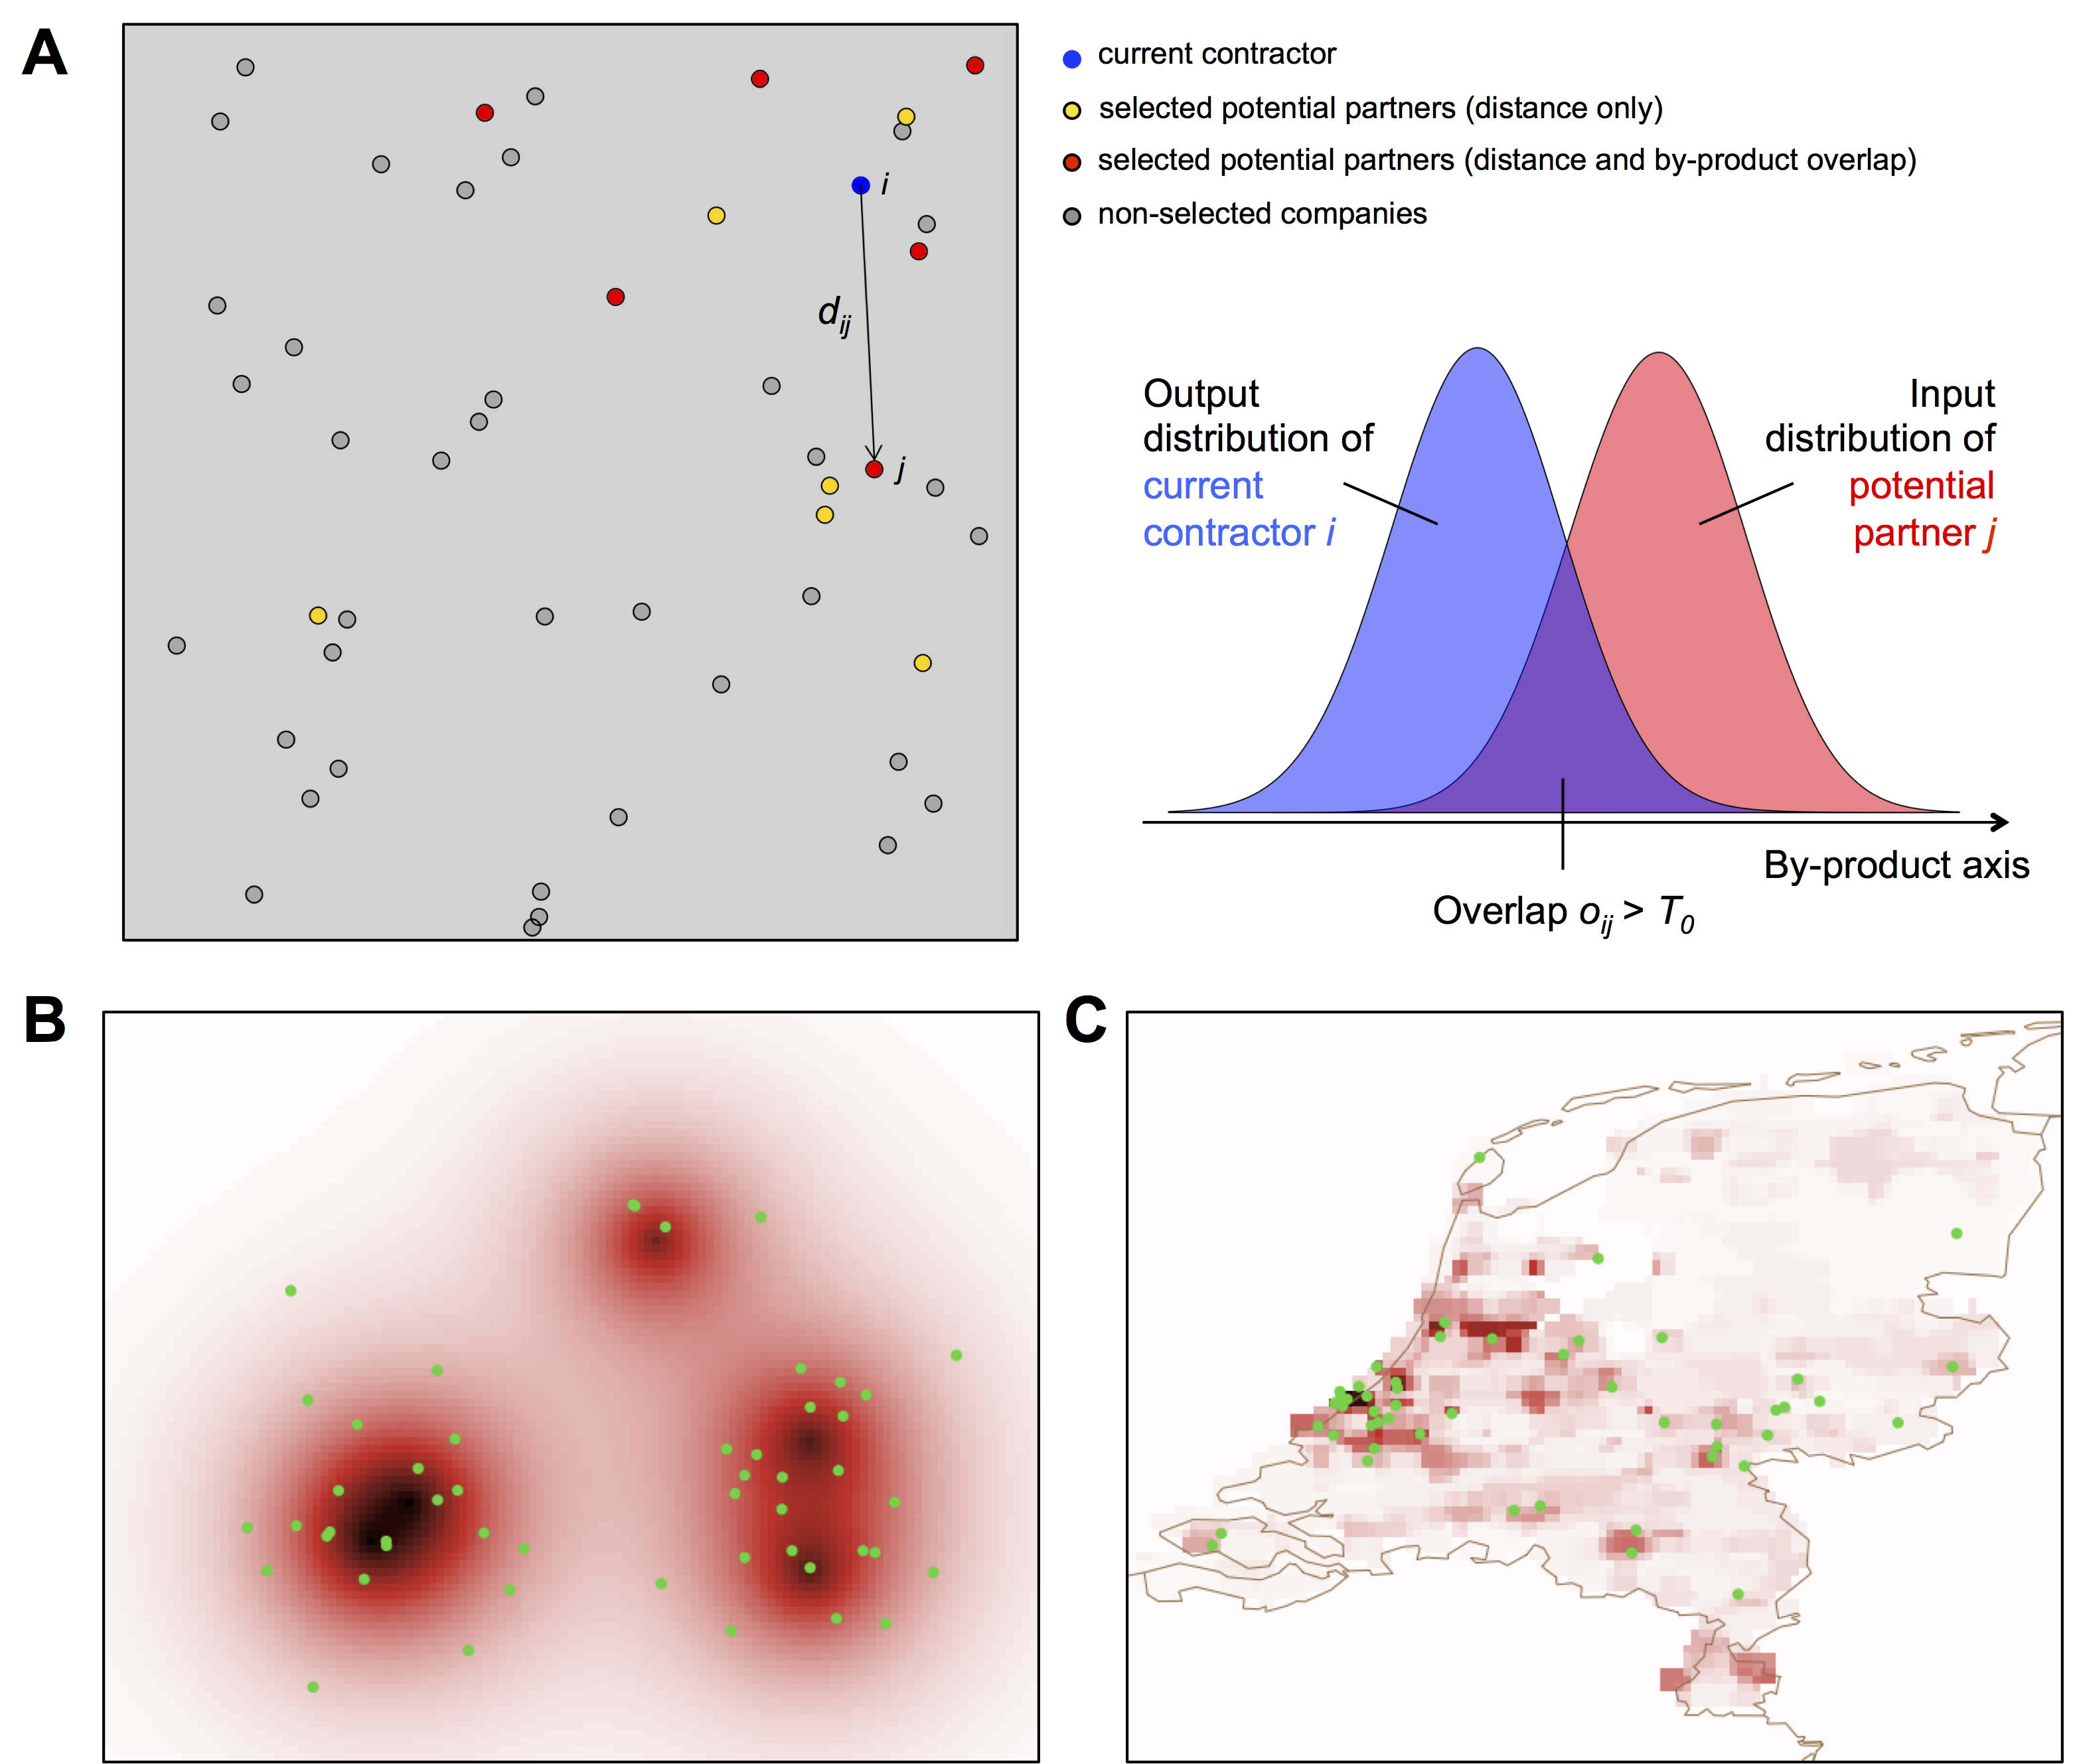
\includegraphics[height=0.85\textheight]{figures/Fig1.png}
\end{center}

}

\sframe{Model description}{

\textbf{Setup: } Companies located into space (synthetic or real setup), with input/output product distribution (Probabilistic Niche Model) which average is correlated with a clustering parameter $\alpha$

\medskip

\textbf{Network growth: } At each time step,
\begin{enumerate}
	\item A current contractor is drawn among companies with minimal number of links.
	\item Spatial interaction model (span $d_0$) determines potential partners.
	\item Partner with the best utility (linear in product overlap and transportation cost) is chosen, link created and distributions updated.
\end{enumerate}

\medskip 

Iterate until the network stabilizes. 

\medskip

\textbf{Indicators: } Total remaining waste (non exchanged products) and relative cost (network length weighted by flows).

}

\sframe{Processes and parameters}{

\begin{center}
\footnotesize
	\begin{tabular}{|l|l|l|l|l|l|}
	\hline
	Parameter & Notation & Process & Range & Value \\ \hline
	Number of firms & $N$ & Economic system & $\left[2 ; 10^6\right]$ & $N \textrm{ = } 50$\\ 
	Hierarchy of city system & $\gamma$ & City system & $\left[0.5 ; 2.0\right]$ & $\gamma \textrm{ = } 1.3$ \\ 
	Density-to-firms exponent & $\alpha_P$ & Economic system & $\left[0.1 ; 4.0\right]$ & $\alpha_P \textrm{ = } 1.5$ \\
	Number of centers & $p$ & City system & $\left[1 ; 10\right]$ & $p \textrm{ = } 5$  \\\hline
	Gravity decay & $d_0$ & Spatial interactions & $\left[1;200\right]$ & $d_0 \textrm{ = } 50 km$ \\
	Distribution width & $\sigma$ & Industrial structure & $\left[0.01 ; 0.1\right]$ & $\sigma \textrm{ = } 0.05$ \\
	Overlap threshold & $T_0$ & Industrial structure & $\left[0.01 ; 0.1\right]$ & $T_0 \textrm{ = } 0.1$ \\
	Transportation cost & $c$ & Urban system & $\left[0.1 ; 4.0\right]$ & $c \textrm{ = } 0.5$ \\
	Correlation level & $\alpha$ & Industrial clusters & $\left[0 ; 20.0\right]$ & $\alpha \textrm{ = } 5$ \\\hline
	\end{tabular}
		
\end{center}



}



\section{Results}

\sframe{Examples of generated networks}{

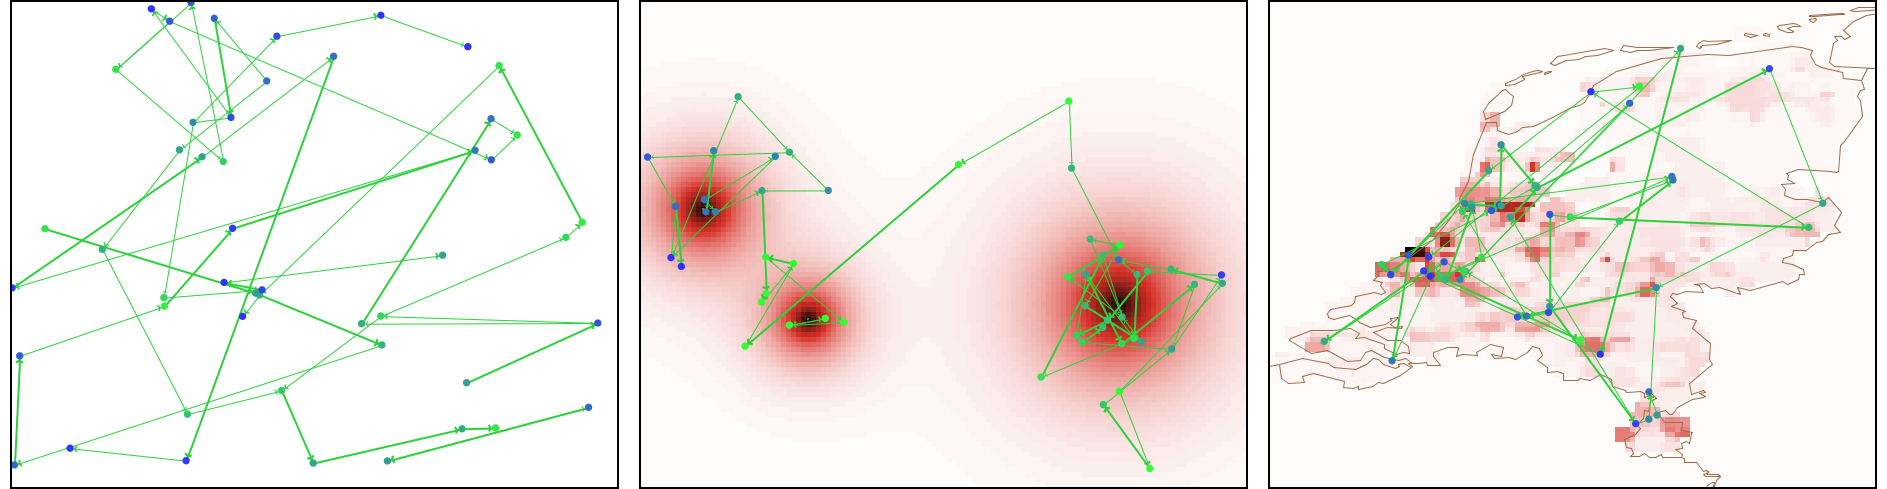
\includegraphics[width=\textwidth]{figures/Fig2.png}

\medskip

\textit{Random company positions, synthetic urban system (scaling law of population), and real population distribution.}

\medskip

\textbf{Model demonstration}


}


\sframe{Model implementation and exploration}{

\justify

\textit{Spatial model with several parameters}

$\rightarrow$ model implemented in NetLogo for its compromise between performance and interactivity

\bigskip

\textit{Consequent number of parameters and processes}



$\rightarrow$ integration into the OpenMOLE model exploration open source software \cite{reuillon2013openmole} 

\url{https://next.openmole.org}

\bigskip

\begin{center}

\includegraphics[height=0.13\textheight]{figures/iconOM.png}

\includegraphics[height=0.13\textheight]{figures/openmole.png}
\end{center}



\textit{Enables seamlessly (i) model embedding; (ii) access to HPC resources; (iii) exploration and optimization algorithms}


}


\sframe{Baseline behavior of the model}{

Running grid sampling on synthetic urban systems with no correlation process:

\begin{itemize}
	\item Statistical consistency of indicators, $n\textrm{=}100$ replications fixed for following experiments.
	\item Expected effect of some parameters, in particular company product span $\sigma$ (decreases waste) and transportation cost $c$ (increases waste and decreases relative cost).
	\item Emerging behaviors: congestion effect with $T_0$ exchange threshold; U-shaped behavior of cost as a function of $\sigma$.
	\item Different qualitative patterns between synthetic and real system for company position setup.
\end{itemize}


}


\sframe{Policy optimization for the circular economy}{

\begin{center}
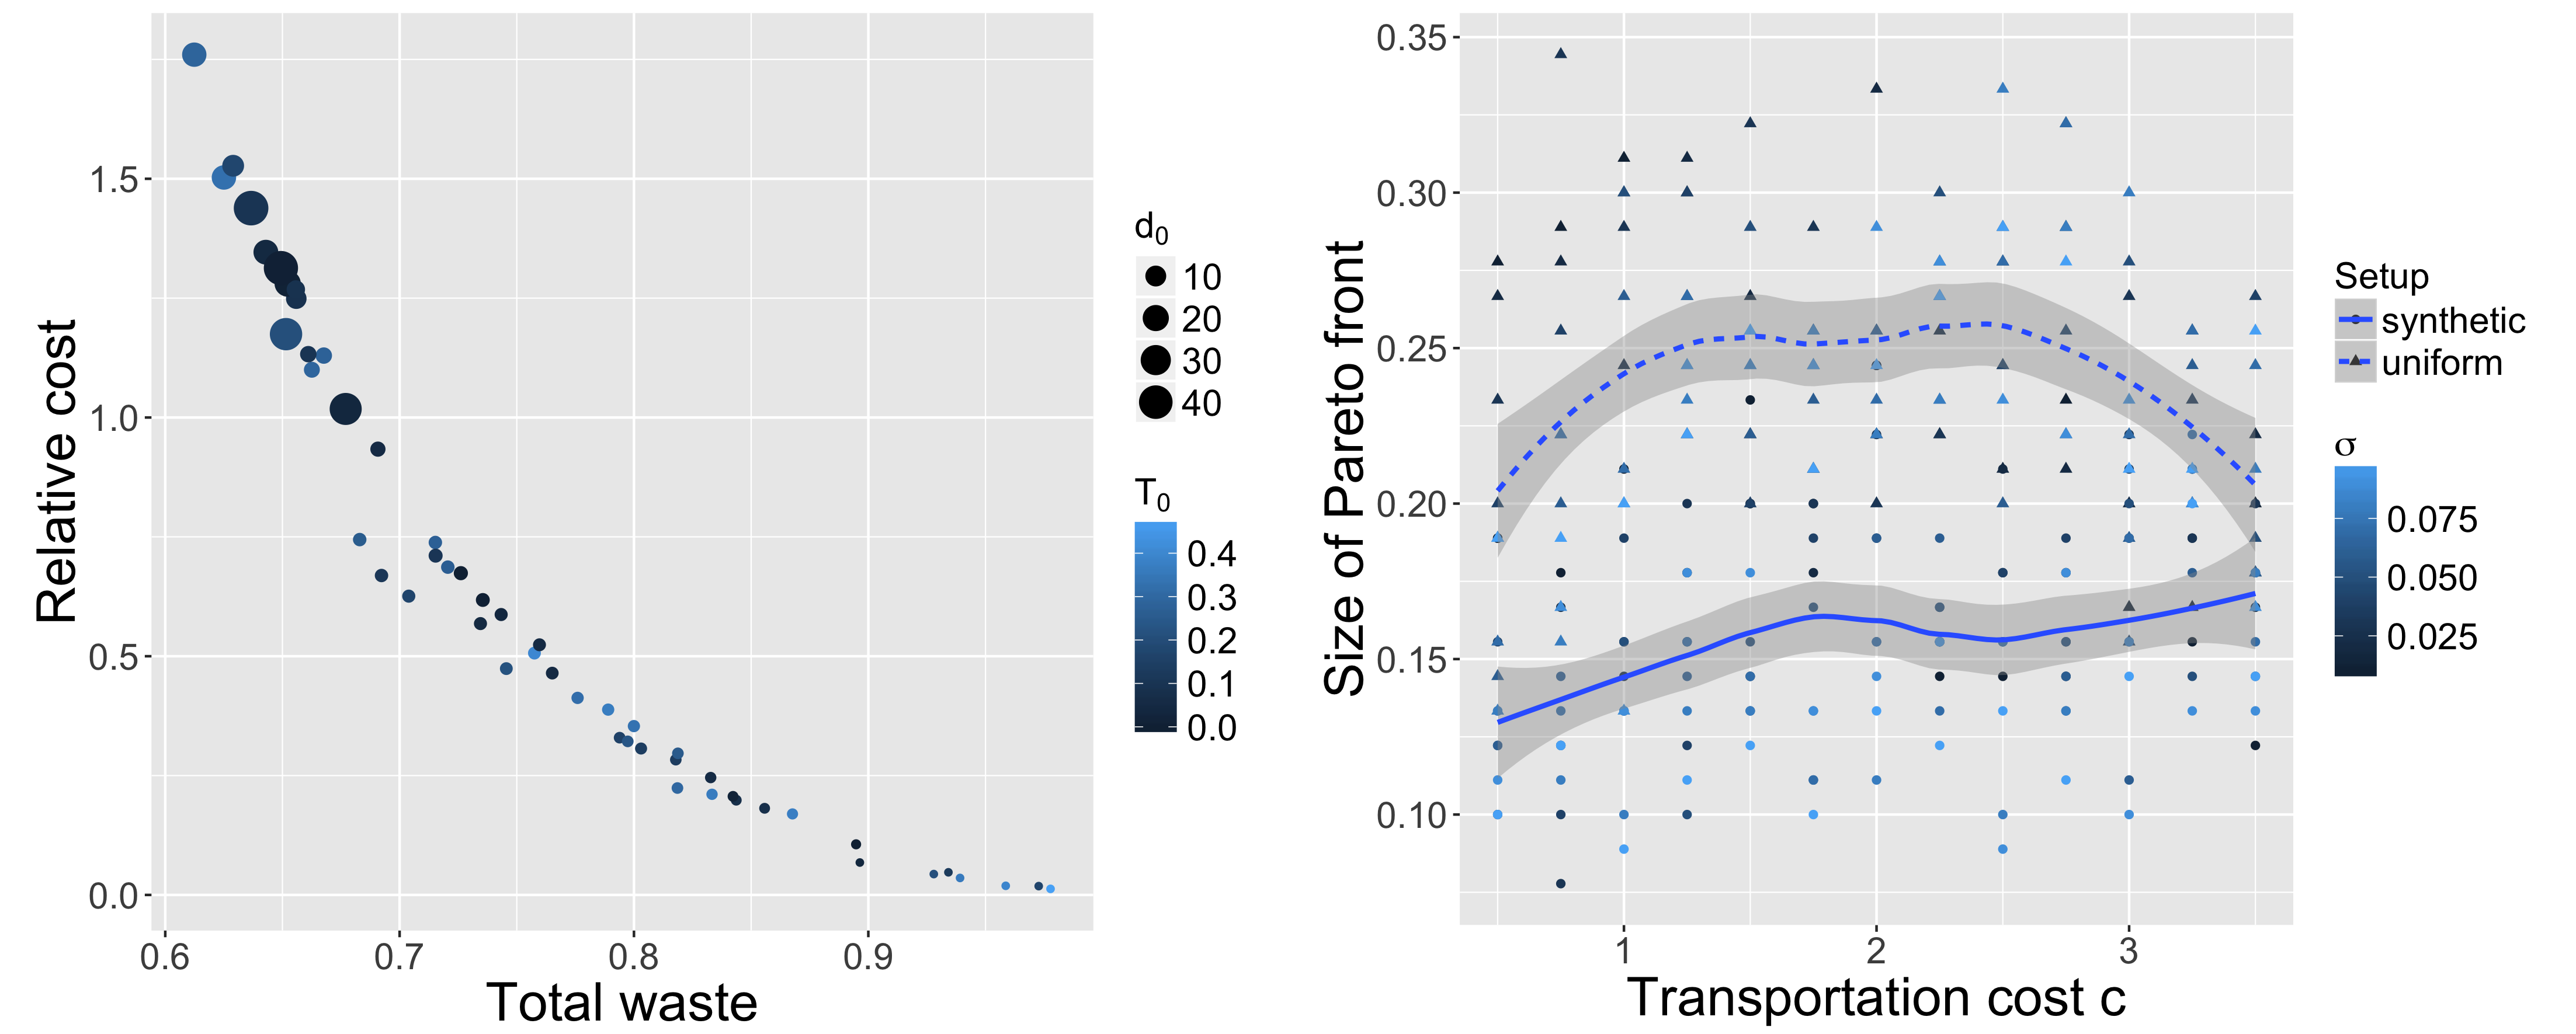
\includegraphics[width=\textwidth]{figures/Fig3.png}
\end{center}

\medskip

\textit{(Left) At fixed exogenous parameters $c$ and $\sigma$, bi-objective optimization of cost and waste; (Right) Size of Pareto fronts (number of alternatives for policy optimization) as a function of $c$ and $\sigma$.}

}


\sframe{Spatial correlation between inputs and outputs}{

\begin{center}
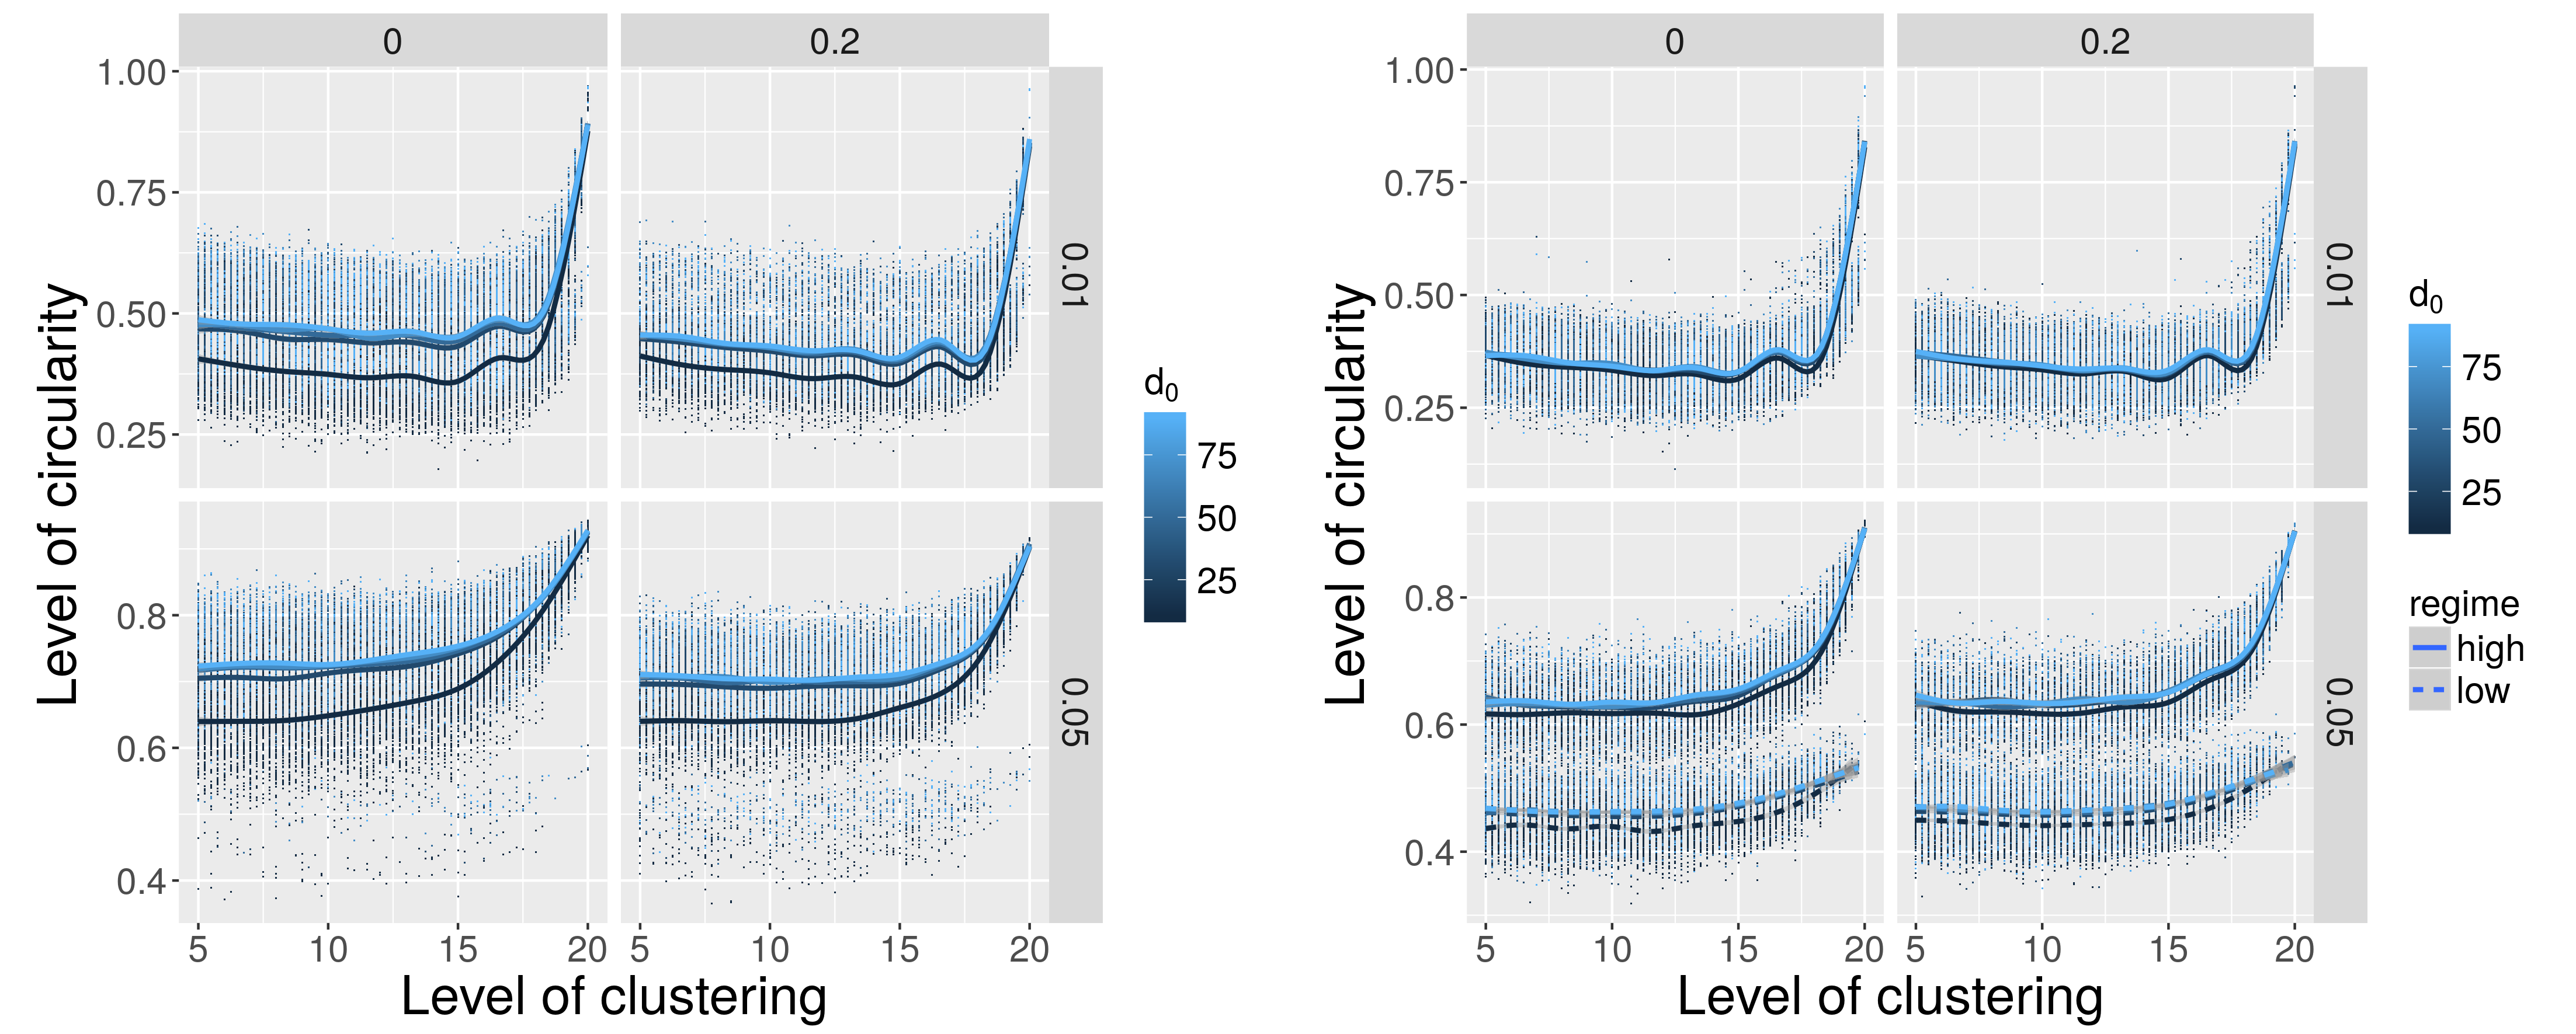
\includegraphics[width=\textwidth]{figures/Fig4.png}
\end{center}

\medskip
\footnotesize

\textit{Influence of level of clustering on the circularity of the final network, for low (resp. high) transportation cost (Left, resp. Right), for different thresholds $T_0$ (columns), distribution width $\sigma$ (rows) and gravity decay $d_0$ (color).}

$\rightarrow$ In practice, the spatial correlation policy must be strictly enforced to have an effect.

}

\sframe{Model calibration}{

\begin{center}
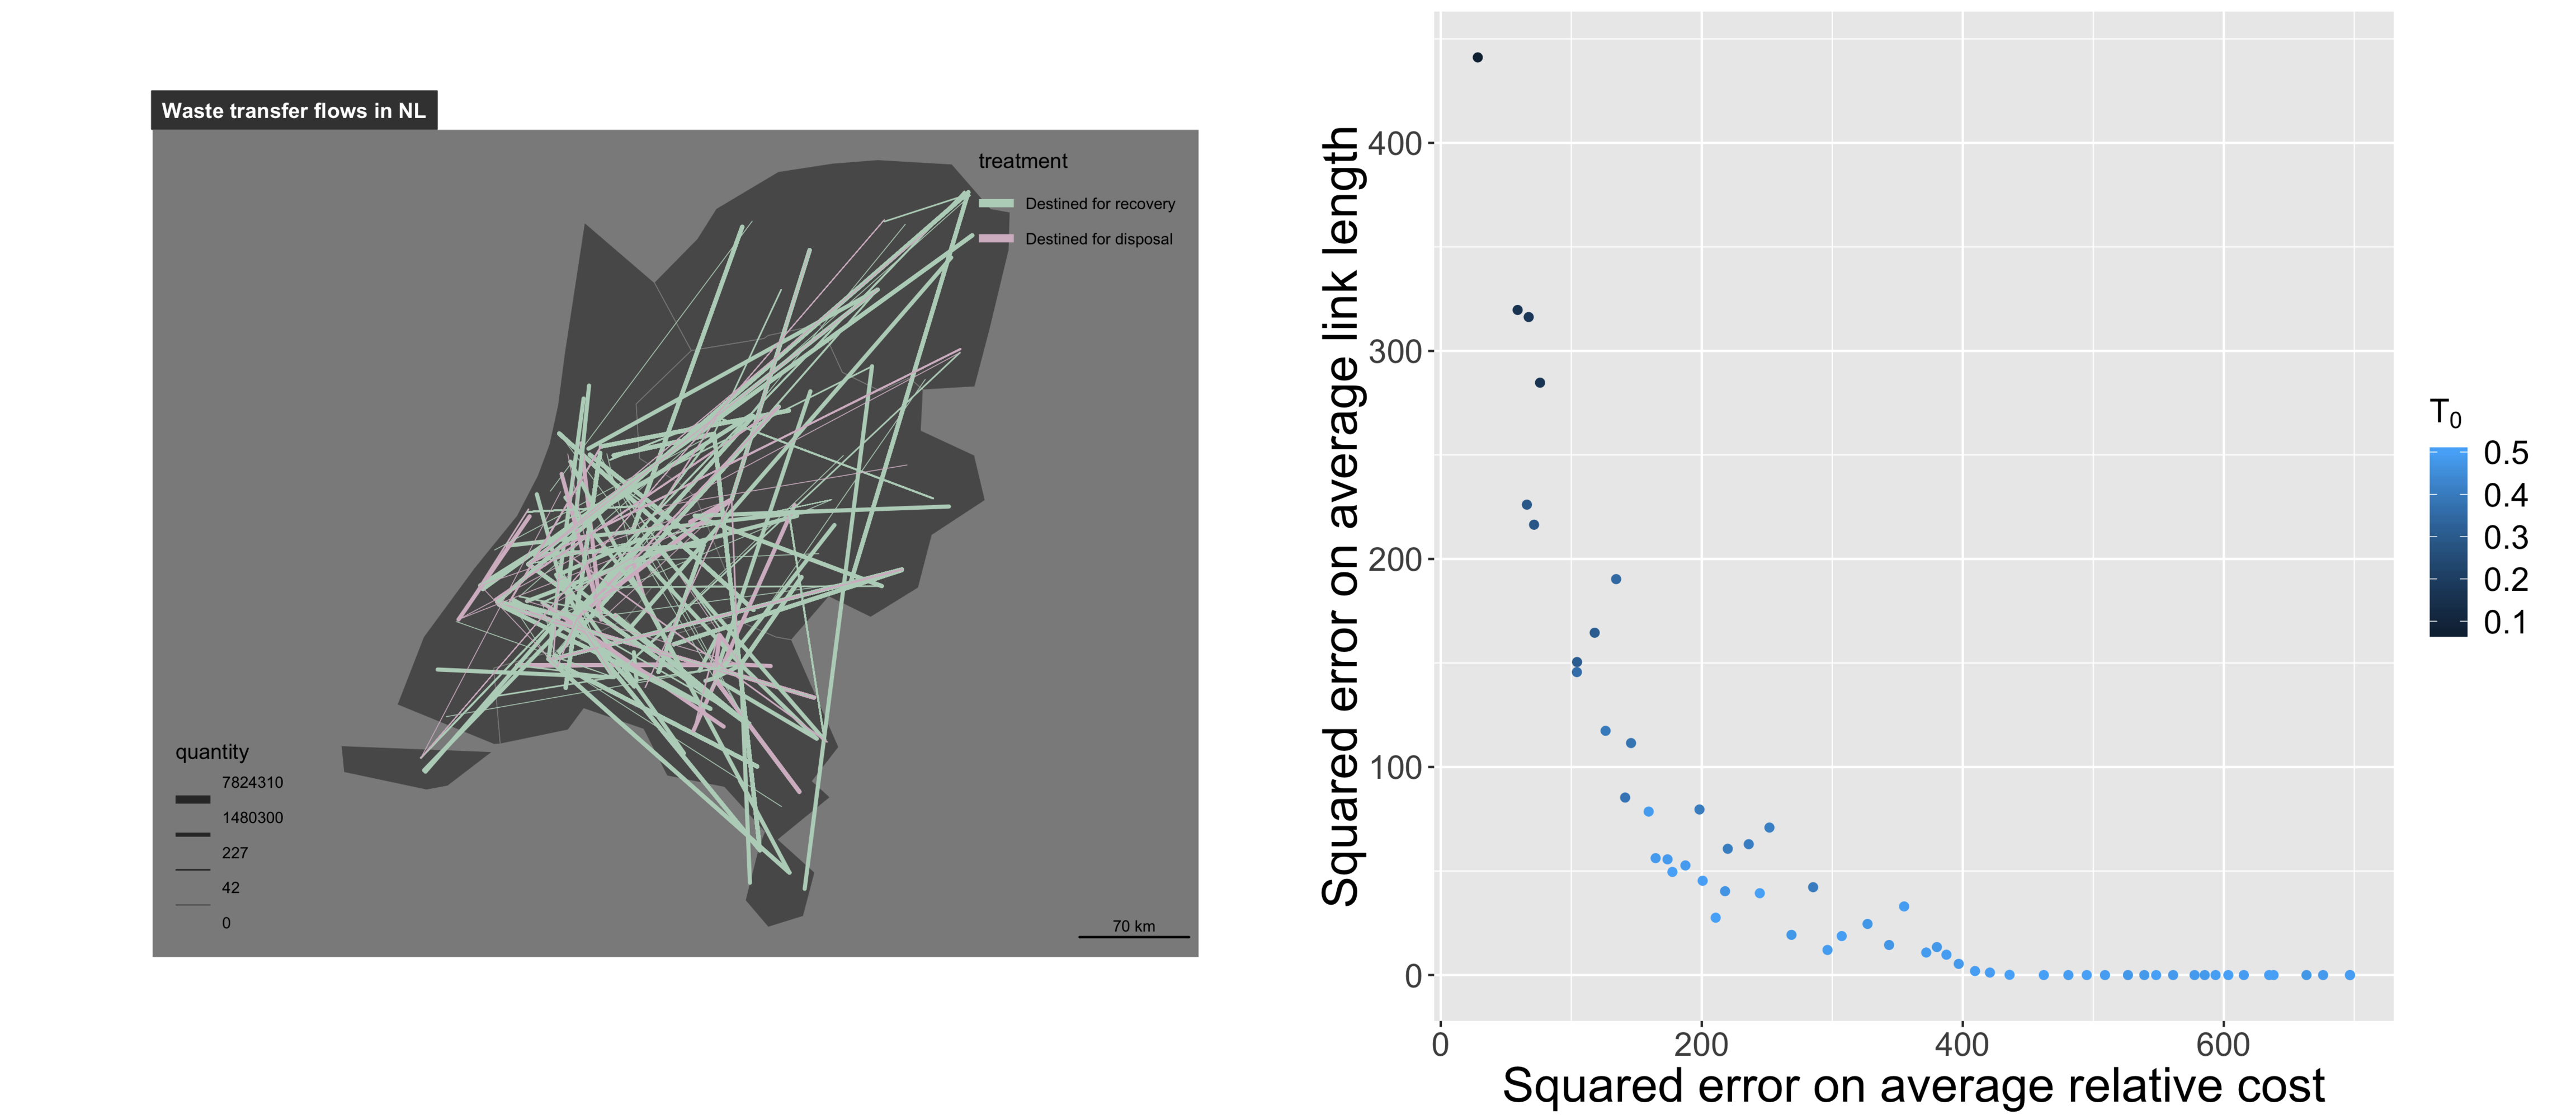
\includegraphics[width=\textwidth]{figures/Fig5.png}
\end{center}

\medskip
\footnotesize

\textit{Real-world application of the model by calibration on the EPRTR database to reproduce network structure (number of links, average link length, relative cost); yield medium range interactions but high propensity to exchange.}

}



\section{Discussion}

\sframe{Discussion}{

\textbf{Implications}

\medskip

$\rightarrow$ Importance of spatial configuration; Eco-industrial park policies must be strictly applied.

\medskip

$\rightarrow$ Real-world application of the model shown as a proof-of-concept with good model fit.

\bigskip

\textbf{Developments}

\medskip

$\rightarrow$ Data-driven approach in link with an interactive web application: towards a real-world application with a project of company.

\medskip

$\rightarrow$ Refinement of economic processes.

\medskip

$\rightarrow$ Benchmark of multiple possible processes and levels of policies.


}


\sframe{Work in progress}{

\justify

\textbf{Multi-modeling}

$\rightarrow$ comparison of several mechanisms to grow networks (self-organisation, intermediaries, central control) \cite{boons2017industrial}

$\rightarrow$ Optimality of hybrid configurations in terms of governance? Role of geographical context and scale?

\bigskip

\textbf{Empirical application}

$\rightarrow$ Companies ownership databases (FAME for UK, AMADEUS for EU): parametrise I/O distributions based on industrial similarity

$\rightarrow$ Stronger probability to cooperate depending on ownership links

\bigskip

\textbf{Towards multi-scale models}

$\rightarrow$ Embed company dynamics into systems of cities models, interaction between industrial symbiosis networks and urban networks  

}



\sframe{Conclusion}{


$\rightarrow$ A simple agent-based model to understand and optimize industrial symbiosis.

\medskip

$\rightarrow$ Important role of spatial structure and spatial correlations.


\bigskip
\bigskip

\footnotesize

\textbf{Git repository: } \texttt{https://github.com/SFICSSS16-CircularEconomy/CircularEconomy}

\bigskip

\textbf{Simulation data: }\texttt{https://doi.org/10.7910/DVN/7XCWTN}% dataverse


\bigskip

\textbf{Acknowledgments}: thanks to the \textit{European Grid Infrastructure} for access to the infrastructure.


}



%%%%%%%%%%%%%%%%%%%%%
\begin{frame}[allowframebreaks]
\frametitle{References}
\bibliographystyle{apalike}
\bibliography{biblio}
\end{frame}
%%%%%%%%%%%%%%%%%%%%%%%%%%%%










\end{document}

